\documentclass[11pt]{article}

\setlength{\topmargin}{0.0in}
\setlength{\oddsidemargin}{0.0in}
\setlength{\evensidemargin}{0.0in}
\setlength{\textwidth}{6.5in}
\setlength{\textheight}{9in}
\setlength{\footskip}{0.5in}
\setlength{\parskip}{0.75em}
\setlength{\parindent}{0in}
\setlength{\voffset}{-0.5in}
\usepackage{graphicx}
\usepackage{amsmath,amssymb}
\usepackage{listings}
\usepackage{needspace}
\usepackage[hidelinks]{hyperref}
\usepackage{xcolor}
\definecolor{codekw}{RGB}{0,82,163}
\definecolor{codecomment}{RGB}{110,110,110}
\definecolor{codestring}{RGB}{163,21,21}
\definecolor{codetype}{RGB}{0,128,96}
\definecolor{codebg}{RGB}{247,247,247}
\lstset{basicstyle=\ttfamily\small,columns=fullflexible,keepspaces=true,breaklines=true,
  keywordstyle=\color{codekw},commentstyle=\color{codecomment}\itshape,
  stringstyle=\color{codestring},showstringspaces=false,upquote=true}
\lstdefinelanguage{Stan}{
  morekeywords={data,parameters,model,generated,quantities,transformed,for,in,if,else,while,return},
  morekeywords=[2]{int,real,vector,array,matrix,lower,upper},
  morekeywords=[3]{normal,log1p_exp,exp,log},
  keywordstyle=[2]\color{codetype},keywordstyle=[3]\color{codekw},
  sensitive=true,morecomment=[l]{//},morecomment=[s]{/*}{*/},morestring=[b]",
  literate={~}{{\raisebox{-0.4ex}{\textasciitilde}}}1}
\lstdefinestyle{code}{backgroundcolor=\color{codebg},frame=single,rulecolor=\color{codebg},
  xleftmargin=0.5em,xrightmargin=0.5em,framesep=4pt}

\newcommand{\T}{\mathsf T}
\emergencystretch=2em
\widowpenalty=10000
\clubpenalty=10000

\begin{document}

{\setlength{\textwidth}{\dimexpr\linewidth-2\fboxsep-2\fboxrule\relax}
\framebox{\begin{minipage}{1.0 \textwidth}
\textit{Computational Methods for Biological Modeling and Simulation (02512/02712)}

\textbf{Name:Jeffrey Wang}

\textbf{Andrew ID: jdw2}

\textbf{AI use statement:}
Improve tricky phrasing when describing reasoning.\\
Reinterpreting question to better understand it. Needed it more for problems 6 and 7.\\
Improving latex code \& formatting.
\end{minipage}}\par}

\begin{center}
{\huge Problem Set 3 }\\
\end{center}

Released Thursday, October 8. Due Thursday, October 29 at 11:59pm US Eastern.
Starred problems are only for 02-712 students.

{\bf Software.} Problem 4 must use Python with the standard library only. Problem 1 uses
CmdStanPy, and Problems 5 and 6 use cvxpy; NumPy and Matplotlib are allowed in those three
problems. Parts that do not ask for code are to be done by hand, though you may use software to
solve linear systems or check your work.
The {\tt PS3-starter} folder has the starting code and {\tt START-HERE.txt}, which
gives installation steps and the commands for each problem. The {\tt PS3-data} folder has the
data files. Submit your written answers, the files you wrote or modified, and your plots. The
\href{https://mc-stan.org/cmdstanpy/installation.html}{CmdStanPy installation guide},
its \href{https://mc-stan.org/cmdstanpy/users-guide/hello_world.html}{first example},
the \href{https://mc-stan.org/docs/reference-manual/blocks.html}{description of Stan program blocks},
and the \href{https://www.cvxpy.org/tutorial/intro/index.html}{cvxpy introduction} are useful
references.

\vspace{0.5em}
\Needspace{18\baselineskip}
{\bf Problem 1 (25 points):} A laboratory follows the growth of a human cell line in culture
and records the cell density $C$, in thousands of cells per mL, every few days. The density
follows a logistic curve with plateau $K>0$, growth rate $r>0$ per day, and halfway day $t_0$,
\[
C_{\rm curve}(t)=\frac{K}{1+\exp[-r(t-t_0)]}.
\]
Measurements scatter multiplicatively around the curve, so that the natural log of each measurement
equals the log of the curve plus an independent normal error with mean zero and unknown
standard deviation $\sigma$. Write $a=\log K$, $\ell=\log r$, and
$m(t)=a-\log(1+\exp[-r(t-t_0)])$ for the log of the curve. Before seeing any data, the lab
gives $a$, $\ell$, and $t_0$ independent normal priors with means $7$, $-1.5$, and $12$ and
standard deviations $3$, $3$, and $10$. For $\sigma$ it uses a half-normal prior with
scale 1, which is the distribution of the absolute value of a normal draw with mean zero and
standard deviation 1.

a. (3 points) Write this description as a generative model. Using the observed log densities
$y_j=\log C_j$ of the readings $C_j$ at days $t_j$, say which quantities are fixed inputs and which are unknown, and write the
priors and the distribution of $y_j$ given the parameters. Give the order of the random draws
needed to simulate a dataset from the full model.
\textcolor{red}{
\begin{itemize}
    \item \textbf{Fixed inputs:} the days $t_1,\dots,t_N$, the number of readings $N$, and the prior means and standard deviations.
    \item \textbf{Observed data:} $y_j = \log C_j$ for $j = 1,\dots,N$.
    \item \textbf{Unknown parameters:} $a, \ell, t_0, \sigma$, with $K = e^{a}$ and $r = e^{\ell}$.
    \item \textbf{Priors:}\\
        $a \sim \text{Normal}(7, 3^2)$\\
        $\ell \sim \text{Normal}(-1.5, 3^2)$\\
        $t_0 \sim \text{Normal}(12, 10^2)$\\
        $\sigma \sim \text{Half-Normal}(0, 1)$
    \item \textbf{Distribution of $y_j$:} independently for each $j$,
        \[ y_j \mid a, \ell, t_0, \sigma \sim \text{Normal}\big(m(t_j), \sigma^2\big), \quad m(t_j) = a - \log\big(1 + \exp[-e^{\ell}(t_j - t_0)]\big). \]
    \item \textbf{Order of draws:}
        \begin{enumerate}
            \item Draw $a$, $\ell$, $t_0$, $\sigma$ from their priors.
            \item Compute $r = e^{\ell}$ and $m(t_j)$ for each day.
            \item For each $j$, draw $y_j \sim \text{Normal}(m(t_j), \sigma^2)$.
        \end{enumerate}
\end{itemize}
}

b. (6 points) Complete the two blocks marked {\tt P1b} in {\tt simulate\_growth.py}. The function
{\tt draw\_parameters} should draw $(a,r,t_0,\sigma)$ from the priors, and
{\tt simulate\_densities} should draw one density for each day given the parameters. Run the
script at its default settings, which fix $K=1200$, $r=0.25$, $t_0=12$, and $\sigma=0.12$, use
seed 3101, and simulate days $0,3,\ldots,30$. Plot log density against day together with $m(t)$.
Check your code in two ways. With {\tt --sigma 0} every point should lie on the curve. With
{\tt --repeats 1000}, report the mean and standard deviation of the log errors $y_j-m(t_j)$ and
compare them with 0 and 0.12. Then simulate five datasets with {\tt --from-prior}, using seeds 1
through 5, and plot them. Using your five draws, describe the range of growth curves these priors
allow.

\textcolor{red}{
\begin{center}
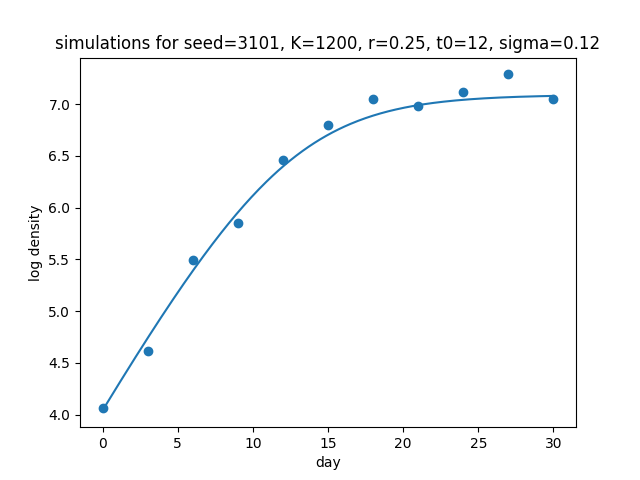
\includegraphics[width=0.48\textwidth]{p1b_simulated.png}
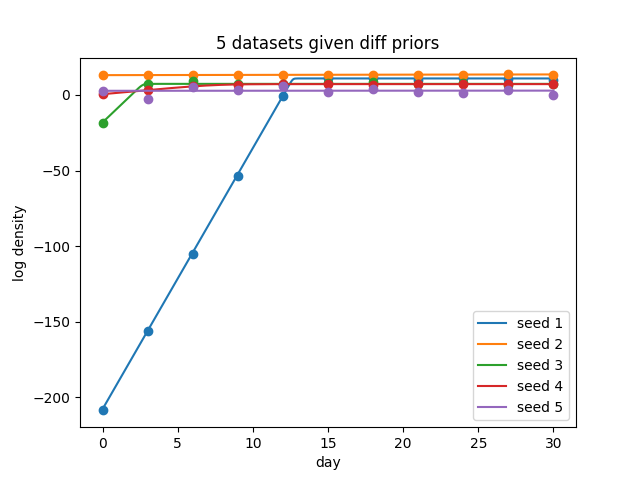
\includegraphics[width=0.48\textwidth]{p1b_prior.png}
\end{center}
\textbf{Check:} \\
{\tt --sigma 0} shows the largest gap between $y_j$ and $m(t_j)$ is exactly 0 $\rightarrow$ every
point lies on the curve\\
{\tt --repeats 1000} the log errors have
$\mu = -0.0009 \approx 0$ and $\sigma = 0.1194 \approx 0.12$\\
\textbf{Prior draw:}
\begin{center}
\begin{tabular}{ccccc}
seed & $K$ & $r$ (per day) & $t_0$ (day) & $\sigma$ \\ \hline
1 & 52{,}300 & 17.3 & 12.7 & 0.77 \\
2 & 1{,}220{,}000 & 0.031 & 15.9 & 0.15 \\
3 & 1{,}460 & 9.49 & 2.7 & 0.99 \\
4 & 1{,}240 & 0.90 & 7.4 & 0.35 \\
5 & 31.9 & 0.0071 & 18.7 & 2.29
\end{tabular}
\end{center}
The plateau ranges from about 30 to 1.2 million (thousands of cells per mL), and the rate ranges from 0.007 to 17 per day. The noise ranges from about 15\% to a factor of $e^{2.29}\approx 10$. These priors allow curves like seed 4, which looks like our simulation, but they also allow many that are not biologically plausible.
}

c. (4 points) Fit {\tt growth\_base.stan} to your seed-3101 dataset with {\tt fit\_growth.py}.
For each line of your model in (a), identify the corresponding statement in the Stan file. Report
the posterior means and 90\% intervals for $K$, $r$, $t_0$, and $\sigma$ next to the values used
in the simulation. The intervals are the {\tt q05} and {\tt q95} columns of {\tt summary.csv},
and the rows {\tt exp(a)} and {\tt exp(logr)} give $K$ and $r$.
Did the fit recover them?

\textcolor{red}{
\textbf{Model to\ Stan line-by-line:}
\begin{center}
\begin{tabular}{ll}
Model (a) & {\tt growth\_base.stan} \\ \hline
Fixed inputs $N$, $t_j$; observed $y_j$ & {\tt data \{ int N; vector[N] t; vector[N] y; \}} \\
Unknowns $a,\ell,t_0$ & {\tt parameters \{ real a; real logr; real t0;} \\
Unknown $\sigma>0$ & {\tt real<lower=0> sigma; \}} \\
$a\sim \text{Normal}(7,3^2)$ & {\tt a $\sim$ normal(7, 3);} \\
$\ell\sim \text{Normal}(-1.5,3^2)$ & {\tt logr $\sim$ normal(-1.5, 3);} \\
$t_0\sim \text{Normal}(12,10^2)$ & {\tt t0 $\sim$ normal(12, 10);} \\
$\sigma\sim \text{Half-Normal}(0,1)$ & {\tt sigma $\sim$ normal(0, 1);} with {\tt <lower=0>} \\
$m(t_j)=a-\log(1+e^{-r(t_j-t_0)})$ & {\tt real m = a - log1p\_exp(-exp(logr) * (t[n] - t0));} \\
$y_j\sim \text{Normal}(m(t_j),\sigma^2)$ & {\tt y[n] $\sim$ normal(m, sigma);}
\end{tabular}
\end{center}
\textbf{Posterior vs.\ true values:}
\begin{center}
\begin{tabular}{lccc}
Parameter & Posterior mean & 90\% interval & True value  \\ \hline
$K$ & 1324 & (1188, 1488) & 1200\\
$r$ & 0.251 & (0.221, 0.279) & 0.25\\
$t_0$ & 12.50 & (11.24, 13.99) & 12\\
$\sigma$ & 0.123 & (0.079, 0.193) & 0.12
\end{tabular}
\end{center}
Yes, the fit recovered them because every true value lies inside its 90\% interval, some of which are almost the exact same value.
}

d. (7 points) The file {\tt growth.json} has measurements from twelve cell lines, in the parallel
lists {\tt cell\_line} (1 through 12), {\tt day}, and {\tt density}. Extend the model so that each
cell line $i$ has its own log plateau $a_i$ and log rate $\ell_i$. Across cell lines, the $a_i$
are normal with unknown mean $\mu_a$ and standard deviation $\tau_a$, and the $\ell_i$ are normal
with unknown mean $\mu_\ell$ and standard deviation $\tau_\ell$, all independent given these
population parameters. The halfway day $t_0$ and measurement standard deviation $\sigma$ are
shared by all cell lines and keep their priors. Give $\mu_a$ and $\mu_\ell$ the priors used for $a$
and $\ell$ before, and give $\tau_a$ and $\tau_\ell$ independent half-normal priors with scale 1. In Stan, keep the names {\tt a}, {\tt logr}, {\tt t0}, and {\tt sigma}, and call the
four new parameters {\tt mu\_a}, {\tt mu\_logr}, {\tt tau\_a}, and {\tt tau\_logr}.

Write the extended generative model. Then edit the blocks marked {\tt P1d} in
{\tt growth\_extend.stan}, which starts as a copy of the base model with the data block already
extended. Run it on {\tt growth.json} and report means and 90\% intervals for $e^{\mu_a}$,
$e^{\mu_\ell}$, $\tau_a$, $t_0$, and $\sigma$ (the rows {\tt exp(mu\_a)} and {\tt exp(mu\_logr)} give
the first two). Explain what $\sigma$ and $\tau_a$ each
describe.

\textcolor{red}{
\textbf{Extended generative model:} We still know the days $t_j$ and cell line $c_j \in \{1,\dots,12\}$ for each
reading $j$. Now the unknowns are $\mu_a, \mu_\ell, \tau_a, \tau_\ell, \{a_1,\dots,a_{12}\}, \{\ell_1,\dots,\ell_{12}\}, t_0, \sigma$.\\
\begin{align*}
&\mu_a \sim \text{Normal}(7, 3^2), \quad \mu_\ell \sim \text{Normal}(-1.5, 3^2), \quad \tau_a, \tau_\ell \sim \text{Half-Normal}(0, 1), \\
&t_0 \sim \text{Normal}(12, 10^2), \quad \sigma \sim \text{Half-Normal}(0, 1), \\
&a_i \mid \mu_a, \tau_a \sim \text{Normal}(\mu_a, \tau_a^2), \quad \ell_i \mid \mu_\ell, \tau_\ell \sim \text{Normal}(\mu_\ell, \tau_\ell^2), \quad i = 1,\dots,12, \\
&y_j \mid \cdot \sim \text{Normal}\big(m_j, \sigma^2\big), \quad \text{where } m_j = a_{c_j} - \log\big(1 + \exp[-e^{\ell_{c_j}}(t_j - t_0)]\big).
\end{align*}
Draw the population parameters, $t_0$ and $\sigma$, then each $a_i$ and $\ell_i$, then each $y_j$.\\
\textbf{Results:}
\begin{center}
\begin{tabular}{lcc}
 & Mean & 90\% interval \\ \hline
$e^{\mu_a}$ & 1186 & (993, 1405) \\
$e^{\mu_\ell}$ & 0.220 & (0.181, 0.264) \\
$\tau_a$ & 0.344 & (0.233, 0.504) \\
$t_0$ & 11.94 & (11.55, 12.35) \\
$\sigma$ & 0.121 & (0.108, 0.136)
\end{tabular}
\end{center}
$\sigma$ is the measurement noise within a cell line on the log scale. $\sigma = 0.121$ means readings are off by about 12.1\%.\\
$\tau_a$ is the variation between cell lines. $\tau_a = 0.344$ means a typical line's plateau is within a factor of about $e^{0.344} \approx 1.41$ of the population plateau $e^{\mu_a}$.
}

e. (5 points) Cell line 12 has only four readings, all taken by day 9. Compare the plateau
intervals for cell lines 12 and 1 in your extended fit. Where does the extended fit get its
information about cell line 12's plateau, and what assumptions does that information depend on?
If cell line 12 were fit on its own with the base model, would its plateau be unidentified, or
only weakly informed by its four readings? Explain using the shape of the curve before day 9.

\textcolor{red}{
\begin{center}
\begin{tabular}{lcc}
Cell line & Mean $K_i$ & 90\% interval \\ \hline
1 & 1474 & (1369, 1586) \\
12 & 1573 & (1283, 1895)
\end{tabular}
\end{center}
Line 12's interval is about 3 times wider than line 1's (612 vs.\ 217) because line 1 has readings on its plateau (days 18--30), while line 12 stops at day 9, before the halfway day.\\
\textbf{Where the information comes from:} the other eleven lines. They estimate $\mu_a$ and $\tau_a$, which act as a prior for $a_{12}$, and they pin down the shared $t_0 \approx 11.9$. With $t_0$ known, the four early readings tell how far below the plateau the curve still is. This assumes line 12 comes from the same population as the other lines, shares their $t_0$ and $\sigma$, and keeps following the logistic curve after day 9.\\
\textbf{Line 12 only:} weakly informed because before $t_0$, $\log C \approx (a - r t_0) + r t$ is nearly a straight line, so the readings fix the slope and intercept but not $a$ and $t_0$ separately. A larger $K$ with a later $t_0$ fits almost as well. The curve bends slightly as it nears $t_0$, so the data still say a little about $K$. Fitting line 12 alone gives $K$ in (415, 5524), much narrower than the prior but far wider than the pooled interval.
}

\vspace{0.5em}
\Needspace{15\baselineskip}
{\bf Problem 2 (15 points):} In this problem we apply the zero-finding methods from class to a
hypothetical molecular design question. A charged nanoparticle sits inside a synthetic nanopore
whose two ends carry fixed surface charges, and we treat the pore as a one-dimensional channel
in which the particle can move. The particle has effective charge $+1$ in arbitrary units. The
left mouth of the pore, at $x=-1.5$, carries charge $+2$, and the right mouth, at $x=2$, carries
charge $+1.5$, so both mouths repel the particle. A simple model for the potential energy at axial position $x$ is
\[
E(x)=\frac{2}{x+1.5}-\frac{1.5}{x-2}.
\]
The singularities at the two mouths lie outside the interval $[-1,1]$ studied below, so we
ignore them. We want to estimate the
minimum-energy position of the particle by finding a zero of $F(x)=E'(x)$.

Bisection starts from an interval where $F$ has opposite signs at the two endpoints, evaluates
$F$ at the midpoint, and retains the half whose endpoints still differ in sign. The secant
method needs no derivative and keeps no interval.
From the two most recent estimates it takes the zero of the line through
$(x_{k-1},F(x_{k-1}))$ and $(x_k,F(x_k))$,
\[
x_{k+1}=x_k-F(x_k)\frac{x_k-x_{k-1}}{F(x_k)-F(x_{k-1})}.
\]
Newton--Raphson uses the tangent line instead, $x_{k+1}=x_k-F(x_k)/F'(x_k)$. For each method
below, report the final estimate $\hat x$ and two error measures. The forward error
$|\hat x-x^*|$ is the distance from the true zero $x^*$. For this exercise, report a bound or estimate without solving for $x^*$ exactly. For
bisection, use the largest distance from $\hat x$ to a point of the interval it was computed
from, and for the secant and Newton--Raphson methods, use the size of the last update. The backward error $|F(\hat x)|$ is
the amount by which $F$ would have to be shifted for $\hat x$ to be an exact zero.

a. (2 points) Derive $F(x)=E'(x)$, and explain why the minimum-energy position must be a zero
of $F$.

\textcolor{red}{
$F(x) = E'(x) = -\frac{2}{(x+1.5)^2} + \frac{1.5}{(x-2)^2}$\\
$E \to +\infty$ at both mouths, so it has a minimum inside $(-1.5, 2)$, and at an interior minimum the slope is zero. Since $E''(x) = \frac{4}{(x+1.5)^3} - \frac{3}{(x-2)^3} > 0$ on $(-1.5, 2)$, $F$ is increasing and this zero is the only one.
}

b. (4 points) The particle must lie in $[-1,1]$. Perform three iterations of the bisection
method on this interval, showing your work. The final estimate is the third midpoint you
compute, not the midpoint of the interval that remains.

\textcolor{red}{
Start with $[a, b] = [-1, 1]$, where $F(-1) = -8 + \tfrac{1.5}{9} = -7.833 < 0$ and $F(1) = -\tfrac{2}{6.25} + 1.5 = 1.18 > 0$.
\begin{center}
\begin{tabular}{ccccccc}
Iter. & $a$ & $b$ & midpoint $m$ & $F(m)$ & sign & new interval \\ \hline
1 & $-1$ & $1$ & $0$ & $-\tfrac{2}{2.25} + \tfrac{1.5}{4} = -\tfrac{37}{72} = -0.5139$ & $-$ & $[0, 1]$ \\
2 & $0$ & $1$ & $0.5$ & $-\tfrac{2}{4} + \tfrac{1.5}{2.25} = \tfrac{1}{6} = 0.1667$ & $+$ & $[0, 0.5]$ \\
3 & $0$ & $0.5$ & $0.25$ & $-\tfrac{2}{3.0625} + \tfrac{1.5}{3.0625} = -\tfrac{8}{49} = -0.1633$ & $-$ & $[0.25, 0.5]$
\end{tabular}
\end{center}
$\hat x = 0.25$\\
Forward error: $|\hat x - x^*| \le 0.25$ (farthest point of $[0, 0.5]$)\\
Backward error: $|F(\hat x)| = 8/49 \approx 0.163$
}

c. (3 points) Perform three iterations of the secant method starting from $x_0=-1$ and
$x_1=1$, showing your work.

\textcolor{red}{
Using $x_{k+1} = x_k - F(x_k)\dfrac{x_k - x_{k-1}}{F(x_k) - F(x_{k-1})}$, with $F(x_0) = F(-1) = -7.8333$ and $F(x_1) = F(1) = 1.18$:
\begin{align*}
x_2 &= 1 - 1.18\cdot\frac{1 - (-1)}{1.18 - (-7.8333)} = 1 - \frac{2.36}{9.0133} = \frac{499}{676} = 0.73817, & F(x_2) &= 0.54283, \\
x_3 &= 0.73817 - 0.54283\cdot\frac{0.73817 - 1}{0.54283 - 1.18} = 0.73817 - 0.22306 = 0.51510, & F(x_3) &= 0.18776, \\
x_4 &= 0.51510 - 0.18776\cdot\frac{0.51510 - 0.73817}{0.18776 - 0.54283} = 0.51510 - 0.11796 = 0.39714, & F(x_4) &= 0.02816.
\end{align*}
$\hat x = x_4 = 0.3971$\\
Forward error: $|x_4 - x_3| \approx 0.118$\\
Backward error: $|F(\hat x)| \approx 0.0282$
}

d. (4 points) Starting from $x_0=0$, perform three iterations of the Newton--Raphson method,
showing your work.

\textcolor{red}{
$F'(x) = \dfrac{4}{(x+1.5)^3} - \dfrac{3}{(x-2)^3}$, $x_{k+1} = x_k - F(x_k)/F'(x_k)$
\begin{center}
\begin{tabular}{cccccc}
$k$ & $x_k$ & $F(x_k)$ & $F'(x_k)$ & update $-F/F'$ & $x_{k+1}$ \\ \hline
0 & $0$ & $-0.513889$ & $1.560185$ & $+0.329377$ & $0.329377$ \\
1 & $0.329377$ & $-0.060173$ & $1.296764$ & $+0.046402$ & $0.375779$ \\
2 & $0.375779$ & $1.759\times10^{-4}$ & $1.306201$ & $-1.347\times10^{-4}$ & $0.375644$
\end{tabular}
\end{center}
$\hat x = x_3 = 0.375644$\\
Forward error: $|x_3 - x_2| \approx 1.35\times10^{-4}$\\
Backward error: $|F(\hat x)| \approx 2.9\times10^{-9}$
}

e. (2 points) Evaluate $E$ at each final estimate. Rank the methods by each error measure
and by energy.

\textcolor{red}{
\begin{center}
\begin{tabular}{lcccc}
Method & $\hat x$ & Forward error & Backward error $|F(\hat x)|$ & $E(\hat x)$ \\ \hline
Bisection & $0.25$ & $\le 0.25$ & $0.163$ & $\tfrac{2}{1.75} + \tfrac{1.5}{1.75} = 2.000000$ \\
Secant & $0.397143$ & $\approx 0.118$ & $0.0282$ & $1.990046$ \\
Newton--Raphson & $0.375644$ & $\approx 1.35\times10^{-4}$ & $2.9\times10^{-9}$ & $1.989743$
\end{tabular}
\end{center}
Forward error, backward error, and energy all rank the methods the same, best to worst: Newton--Raphson, secant, bisection. The energies are much closer than the positions because $E$ is flat near its minimum.
}

\vspace{0.5em}
\Needspace{15\baselineskip}
{\bf Problem 3 (10 points):} We have been monitoring new COVID cases at two-week intervals
and need estimates at a finer time resolution, to test how specific events might have
contributed to the spread. The measurements are
\begin{center}
\begin{tabular}{|c|c|c|c|c|} \hline
$t$ (weeks) & 0 & 2 & 4 & 6\\ \hline
new cases $C$ (thousands) & 0.5 & 1.7 & 3.5 & 10.1\\ \hline
\end{tabular}
\end{center}
and we want estimates for weeks 1, 3, and 5. For each method below, give the interpolating
function or functions on $[0,6]$ and the values they predict at $t=1$, 3, and 5.

a. (2 points) Piecewise linear interpolation.

\textcolor{red}{
Slopes are $\tfrac{1.7-0.5}{2} = 0.6$, $\tfrac{3.5-1.7}{2} = 0.9$, and $\tfrac{10.1-3.5}{2} = 3.3$:
\[
L(t) = \begin{cases}
0.5 + 0.6\,t, & 0 \le t \le 2, \\
1.7 + 0.9\,(t-2), & 2 \le t \le 4, \\
3.5 + 3.3\,(t-4), & 4 \le t \le 6.
\end{cases}
\]
$L(1) = 1.1$, $L(3) = 2.6$, $L(5) = 6.8$
}

b. (4 points) A single cubic polynomial through all four points.

\textcolor{red}{
Using Newton's divided differences:
\begin{center}
\begin{tabular}{ccccc}
$t$ & $C$ & 1st & 2nd & 3rd \\ \hline
0 & 0.5 & & & \\
  &     & $\tfrac{1.7-0.5}{2} = 0.6$ & & \\
2 & 1.7 & & $\tfrac{0.9-0.6}{4} = 0.075$ & \\
  &     & $\tfrac{3.5-1.7}{2} = 0.9$ & & $\tfrac{0.6-0.075}{6} = 0.0875$ \\
4 & 3.5 & & $\tfrac{3.3-0.9}{4} = 0.6$ & \\
  &     & $\tfrac{10.1-3.5}{2} = 3.3$ & & \\
6 & 10.1 & & &
\end{tabular}
\end{center}
\begin{align*}
p(t) &= 0.5 + 0.6\,t + 0.075\,t(t-2) + 0.0875\,t(t-2)(t-4) \\
     &= 0.0875\,t^3 - 0.45\,t^2 + 1.15\,t + 0.5.
\end{align*}
$p(1) = 1.2875$, $p(3) = 2.2625$, $p(5) = 5.9375$
}

c. (4 points) A quadratic spline through every data point, with matching first derivatives at $t=2$
and $t=4$ and with $C'(0)=0$ (cases were initially stable). Write the linear system for the nine coefficients and solve it, by hand or with code.

\textcolor{red}{
On each interval $[t_i, t_{i+1}]$ with $t_1 = 0$, $t_2 = 2$, $t_3 = 4$, write $S_i(t) = a_i + b_i(t - t_i) + c_i(t - t_i)^2$,
so $S_i'(t) = b_i + 2c_i(t - t_i)$. The nine conditions are
\begin{align*}
&S_1(0) = a_1 = 0.5, & &S_1(2) = a_1 + 2b_1 + 4c_1 = 1.7, \\
&S_2(2) = a_2 = 1.7, & &S_2(4) = a_2 + 2b_2 + 4c_2 = 3.5, \\
&S_3(4) = a_3 = 3.5, & &S_3(6) = a_3 + 2b_3 + 4c_3 = 10.1, \\
&S_1'(2) = S_2'(2):\ b_1 + 4c_1 - b_2 = 0, & &S_2'(4) = S_3'(4):\ b_2 + 4c_2 - b_3 = 0, \\
&S_1'(0) = b_1 = 0.
\end{align*}
\[
\begin{pmatrix}
1&0&0&0&0&0&0&0&0\\
1&2&4&0&0&0&0&0&0\\
0&0&0&1&0&0&0&0&0\\
0&0&0&1&2&4&0&0&0\\
0&0&0&0&0&0&1&0&0\\
0&0&0&0&0&0&1&2&4\\
0&1&4&0&-1&0&0&0&0\\
0&0&0&0&1&4&0&-1&0\\
0&1&0&0&0&0&0&0&0
\end{pmatrix}
\begin{pmatrix} a_1\\ b_1\\ c_1\\ a_2\\ b_2\\ c_2\\ a_3\\ b_3\\ c_3 \end{pmatrix}
=
\begin{pmatrix} 0.5\\ 1.7\\ 1.7\\ 3.5\\ 3.5\\ 10.1\\ 0\\ 0\\ 0 \end{pmatrix}.
\]
Solving by hand...\\
$a_1 = 0.5$, $b_1 = 0$, $c_1 = 1.2/4 = 0.3$\\
$a_2 = 1.7$, $b_2 = b_1 + 4c_1 = 1.2$, $c_2 = (3.5 - 1.7 - 2.4)/4 = -0.15$\\
$a_3 = 3.5$, $b_3 = b_2 + 4c_2 = 0.6$, $c_3 = (10.1 - 3.5 - 1.2)/4 = 1.35$
\[
S(t) = \begin{cases}
0.5 + 0.3\,t^2, & 0 \le t \le 2, \\
1.7 + 1.2\,(t-2) - 0.15\,(t-2)^2, & 2 \le t \le 4, \\
3.5 + 0.6\,(t-4) + 1.35\,(t-4)^2, & 4 \le t \le 6.
\end{cases}
\]
$S(1) = 0.8$, $S(3) = 2.75$, $S(5) = 5.45$
}

\vspace{0.5em}
\Needspace{15\baselineskip}
{\bf Problem 4 (20 points):} In this programming problem you will fit a recovery-to-plateau
model to noisy data. The model is used in fluorescence recovery after photobleaching (FRAP) and
in other kinetic experiments. In FRAP, molecules are labeled with a fluorescent probe, and the probe is then
deliberately destroyed within a small region of a cell. The mean fluorescence in that region
recovers toward an asymptote as mobile molecules exchange with the bleached ones. A common
approximation for the normalized mean recovery is
\[
R(t)=R_\infty\left(1-e^{-kt}\right),
\]
where $R_\infty\in(0,1]$ is the plateau and $k>0$ is an effective rate constant. Given
observations $(t_i,R_i)$, we estimate $(R_\infty,k)$ by minimizing the sum of squared errors
\[
\Phi(R_\infty,k)=\sum_{i=1}^n\left(R_i-R_\infty\left(1-e^{-kt_i}\right)\right)^2.
\]

a. (3 points) Derive the gradient of $\Phi$, giving closed-form expressions for
$\partial\Phi/\partial R_\infty$ and $\partial\Phi/\partial k$.

\textcolor{red}{
\begin{align*}
\frac{\partial\Phi}{\partial R_\infty} &= -2\sum_{i=1}^n \left(R_i - R_\infty(1 - e^{-kt_i})\right)\left(1 - e^{-kt_i}\right), \\
\frac{\partial\Phi}{\partial k} &= -2R_\infty\sum_{i=1}^n \left(R_i - R_\infty(1 - e^{-kt_i})\right) t_i e^{-kt_i}.
\end{align*}
}

b. (4 points) Rather than derive the analytic Hessian, we approximate it by finite differences.
Give forward-difference formulas, using values of $\Phi$ only, for the three distinct Hessian
entries, with steps $\Delta R$ in $R_\infty$ and $\Delta k$ in $k$. Applying a forward
difference twice gives, for a function $f$ of one variable,
$f''(x)\approx[f(x+2h)-2f(x+h)+f(x)]/h^2$; the mixed entry follows from taking a forward
difference in $R_\infty$ of a forward difference in $k$.

\textcolor{red}{
Given that $R = R_\infty$ we will use the following finite difference approximations for the Hessian entries:
\begin{align*}
\frac{\partial^2\Phi}{\partial R^2} &\approx \frac{\Phi(R + 2\Delta R, k) - 2\Phi(R + \Delta R, k) + \Phi(R, k)}{\Delta R^2}, \\
\frac{\partial^2\Phi}{\partial k^2} &\approx \frac{\Phi(R, k + 2\Delta k) - 2\Phi(R, k + \Delta k) + \Phi(R, k)}{\Delta k^2}, \\
\frac{\partial^2\Phi}{\partial R\,\partial k} &\approx \frac{\Phi(R + \Delta R, k + \Delta k) - \Phi(R + \Delta R, k) - \Phi(R, k + \Delta k) + \Phi(R, k)}{\Delta R\,\Delta k}.
\end{align*}
The Hessian is symmetric, so $\partial^2\Phi/\partial k\,\partial R$ is the same entry.
}

c. (6 points) Give pseudocode for a Newton--Raphson solver that takes a starting point
$(R_{\infty,0},k_0)$, steps $(\Delta R,\Delta k)$, an iteration count $q$, and data vectors
$\vec t$ and $\vec R$, and returns $(R_\infty,k)$ after $q$ iterations. Use the gradient from (a)
and the Hessian from (b).

{\color{red}
\begin{lstlisting}[style=code,basicstyle=\ttfamily\small\color{red},commentstyle=\color{red}\itshape]
function NEWTON(R0, k0, dR, dk, q, t, R):
    (x, y) = (R0, k0)
    repeat q times:
        gx, gy = GRADIENT(x, y, t, R)
        f00 = PHI(x, y)
        Hxx = (PHI(x+2dR, y) - 2 PHI(x+dR, y) + f00) / dR^2
        Hyy = (PHI(x, y+2dk) - 2 PHI(x, y+dk) + f00) / dk^2
        Hxy = (PHI(x+dR, y+dk) - PHI(x+dR, y) - PHI(x, y+dk) + f00) / (dR dk)

        det = Hxx Hyy - Hxy^2
        sx = (-gx Hyy + gy Hxy) / det
        sy = (-gy Hxx + gx Hxy) / det
        (x, y) = (x + sx, y + sy)
    return (x, y)
\end{lstlisting}
}

\Needspace{16\baselineskip}
d. (4 points) Implement your solver in Python with the standard library only. The program
should take the name of an input file as its command-line argument and read a file of the form
\begin{center}
\begin{minipage}{0.3\linewidth}
\begin{lstlisting}
R_inf0
k0
Delta_R
Delta_k
q
n
t_1  R_1
...
t_n  R_n
\end{lstlisting}
\end{minipage}
\end{center}
and print the final estimates {\tt R\_inf k} on one line, separated by a space.

\textcolor{red}{
Run {\tt python frap.py PS3-data/frap\_a.txt}
}

e. (3 points) Run your solver on {\tt frap\_a.txt}, {\tt frap\_b.txt}, and {\tt frap\_c.txt} in
{\tt PS3-data} and report the estimates.
\textcolor{red}{
\begin{center}
\begin{tabular}{lcccccc}
 & $(R_{\infty,0}, k_0)$ & $q$ & $n$ & $\hat R_\infty$ & $\hat k$ & $\Phi$ \\ \hline
{\tt frap\_a.txt} & $(0.7, 0.2)$ & 20 & 10 & 0.848 & 0.502 & $0.000285$ \\
{\tt frap\_b.txt} & $(0.55, 0.6)$ & 25 & 18 & 0.621 & 0.750 & $0.000221$ \\
{\tt frap\_c.txt} & $(0.85, 0.25)$ & 35 & 16 & 0.944 & 0.280 & $0.000295$
\end{tabular}
\end{center}
}

\vspace{0.5em}
\Needspace{18\baselineskip}
{\bf Problem 5 (15 points):} In this problem we use linear programming to design a genomics
experiment. We want to sequence some tissue and can choose a combination of bulk, single-cell,
and spatial sequencing, in amounts $x_1$, $x_2$, and $x_3$. The technologies differ in how
useful their outputs are and in what they cost. We judge one unit of bulk, single-cell, and
spatial sequencing to be worth 1, 2, and 3, respectively, so we want to
\[
\max\ x_1+2x_2+3x_3.
\]
Bulk and single-cell sequencing use tissue, of which we have 3 units. One unit of bulk
needs 1 unit of tissue, and one unit of single-cell needs 2, so
\[
x_1+2x_2\le 3.
\]
Bulk sequencing is cheap enough that we ignore its cost, but each unit of single-cell or spatial
sequencing costs 1 unit of our budget, which is 8 units, so
\[
x_2+x_3\le 8.
\]
Finally, we have a single-cell sequencer in our lab but must send bulk and spatial samples to a
company, which takes time. Bulk takes 2 units of time per unit and spatial takes 1, and we need
the data back within 10 units of time, so
\[
2x_1+x_3\le 10.
\]
We cannot do a negative amount of sequencing, so $x_1,x_2,x_3\ge0$.

A linear program in standard form minimizes $c^\T x$ subject
to $Ax=b$ and $x\ge0$. Each constraint $a^\T x\le\beta$ becomes an equality by adding a
slack variable $s=\beta-a^\T x\ge0$, the unused amount of that resource (here $s_1$, $s_2$, and $s_3$ for
tissue, budget, and time), and a maximization
becomes a minimization by negating the objective. The simplex method starts at a feasible vertex, here
$x=0$ with every slack equal to the right-hand side of its constraint, and writes the slacks and the objective in terms of
the variables that are zero. At each step it chooses a zero variable with a negative objective
coefficient, called the entering variable (for example, the one with the most negative
coefficient), and increases it until another variable, called the
leaving variable, reaches zero. It then solves the leaving variable's equation for
the entering variable and substitutes the result into the other equations and the objective. When no objective coefficient is negative, the current vertex is optimal.

a. (2 points) Convert the linear program to standard form.

\textcolor{red}{
$x = (x_1, x_2, x_3, s_1, s_2, s_3)$ with $s_1$, $s_2$, and $s_3$ the slack variables for tissue, budget, and time, respectively. The linear program becomes...
\[
\min\ -x_1 - 2x_2 - 3x_3 \quad \text{subject to} \quad
\begin{aligned}
x_1 + 2x_2 + s_1 &= 3, \\
x_2 + x_3 + s_2 &= 8, \\
2x_1 + x_3 + s_3 &= 10,
\end{aligned}
\qquad x_1, x_2, x_3, s_1, s_2, s_3 \ge 0.
\]
That is, $c = (-1, -2, -3, 0, 0, 0)^\T$, $b = (3, 8, 10)^\T$, and
$A = [\,A_x \mid I\,] = \left(\begin{array}{ccc|ccc} 1&2&0&1&0&0\\ 0&1&1&0&1&0\\ 2&0&1&0&0&1 \end{array}\right)$.
}

b. (7 points) Solve the linear program by the simplex method, showing your work, to find the
optimal amount of each kind of sequencing.
\textcolor{red}{
\begin{enumerate}
\item $x = 0$ and minimizing the objective $z = -x_1 - 2x_2 - 3x_3$:
\[
s_1 = 3 - x_1 - 2x_2, \qquad s_2 = 8 - x_2 - x_3, \qquad s_3 = 10 - 2x_1 - x_3, \qquad z = -x_1 - 2x_2 - 3x_3 = 0.
\]
\item $x_3$ enters (most negative). \\
Limits: $s_2$: 8, $s_3$: 10, so $s_2$ leaves. \\
Substituting $x_3 = 8 - x_2 - s_2$,
\[
x_3 = 8 - x_2 - s_2, \qquad s_1 = 3 - x_1 - 2x_2, \qquad s_3 = 2 - 2x_1 + x_2 + s_2, \qquad z = -24 - x_1 + x_2 + 3s_2.
\]
\item $x_1$ enters (only negative). \\
Limits: $s_1$: 3, $s_3$: $2/2 = 1$, so $s_3$ leaves. \\
Substituting $x_1 = 1 + \tfrac12 x_2 + \tfrac12 s_2 - \tfrac12 s_3$,
\begin{align*}
x_1 &= 1 + \tfrac12 x_2 + \tfrac12 s_2 - \tfrac12 s_3, & x_3 &= 8 - x_2 - s_2, \\
s_1 &= 2 - \tfrac52 x_2 - \tfrac12 s_2 + \tfrac12 s_3, & z &= -25 + \tfrac12 x_2 + \tfrac52 s_2 + \tfrac12 s_3.
\end{align*}
\item All objective coefficients are nonnegative, so this vertex is optimal:
\[
x_1 = 1 \text{ (bulk)}, \qquad x_2 = 0 \text{ (single-cell)}, \qquad x_3 = 8 \text{ (spatial)}, \qquad s_1 = 2,
\]
with maximum value $x_1 + 2x_2 + 3x_3 = 1 + 24 = 25$.
\end{enumerate}
}

c. (2 points) One of the three resource constraints is not tight at the optimum. Which resource
is in excess, and how much is left over?

\textcolor{red}{
Tissue is in excess. The plan uses $x_1 + 2x_2 = 1$ of 3 units, so $s_1 = 2$ units are left over.
}

d. (4 points) Complete the block marked {\tt P5d} in {\tt sequencing.py} with this linear
program, writing the three resource constraints as a Python list with the function's
arguments {\tt tissue}, {\tt budget}, and {\tt time} as their limits, and run it. The script solves the program and then solves it again with one more unit of
each resource in turn. Report the optimum and the dual values of the three resource constraints.
Compare the dual values with the coefficients of the slack variables in the objective at
your final simplex step, and with the gains in value from the extra units. Explain the dual
value for the resource you identified in (c).
\textcolor{red}{
\begin{center}
\begin{tabular}{lccc}
(tissue, budget, time) & $x$ & Optimum & Gains \\ \hline
$(3, 8, 10)$ & $(1, 0, 8)$ & 25 & -- \\
$(4, 8, 10)$ & $(1, 0, 8)$ & 25 & 0 \\
$(3, 9, 10)$ & $(0.5, 0, 9)$ & 27.5 & 2.5 \\
$(3, 8, 11)$ & $(1.5, 0, 8)$ & 25.5 & 0.5
\end{tabular}
\end{center}
Optimum: $x = (1, 0, 8)$ with value 25, same as (b).\\
Dual values (tissue, budget, time): $(0, 2.5, 0.5)$. These equal the coefficients of $s_1, s_2, s_3$ in the final simplex objective $z = -25 + \tfrac12 x_2 + \tfrac52 s_2 + \tfrac12 s_3$ ($s_1$ is absent, so 0) and the gains from one extra unit of each resource.\\
Tissue's dual value is 0 because 2 units are already unused, so an extra unit cannot change the optimum.
}

\vspace{0.5em}
\Needspace{18\baselineskip}
{\bf Problem 6 (15 points):} Genomic deconvolution explains gene expression measured in a bulk
tissue sample as a mixture of contributions from different cell types. We measure $n$ genes in
a bulk blood sample, giving a vector $\vec v=(v_1,\ldots,v_n)$. We also have reference expression
for $k$ cell types measured separately on the same genes, giving an $n\times k$ matrix $R$ whose
column $j$ is the expression signature of cell type $j$. We want coefficients
$\vec c=(c_1,\ldots,c_k)$ giving the amount of each cell type, so that $R\vec c$ explains
$\vec v$. Assume $n\gg k$ and that the columns of $R$ are linearly independent.
In all parts, allow $\vec c$ to range over $\mathbb R^k$, without imposing nonnegativity or a
sum-to-one constraint.

a. (2 points) We first want the least-squares fit, the $\vec c$ minimizing $\|R\vec c-\vec v\|^2$.
Show how to find it by solving a linear system.

\textcolor{red}{
$\nabla f = 2R^\T R\,\vec c - 2R^\T\vec v = 0 \rightarrow R^\T R\,\vec c = R^\T\vec v$\\
These are the normal equations for the least-squares problem. The solution is then unique because the columns of $R$ are independent, so $R^\T R$ is invertible and $\vec c = (R^\T R)^{-1}R^\T\vec v$ (i.e. there's a bottom).
}

b. (4 points) A least-squares fit tends to assign small amounts, positive or negative, to every
cell type, even to types that are absent, by fitting the noise. One remedy adds a penalty on the sizes of the
coefficients. A variant
that can be posed as a linear program measures both the fit and the penalty with absolute
values:
\[
\min_{\vec c}\ \sum_{i=1}^n|(R\vec c)_i-v_i|+\lambda\sum_{j=1}^k|c_j|
\]
for a constant $\lambda\ge0$. Show how to pose this as a linear program. (Hint: define auxiliary
variables, and note that $x\ge|y|$ if and only if $x\ge y$ and $x\ge-y$.)

\textcolor{red}{
Let $e_i$ stand in for $|(R\vec c)_i - v_i|$ and $u_j$ for $|c_j|$:
\begin{align*}
\min_{\vec c,\,\vec e,\,\vec u}\quad & \sum_{i=1}^n e_i + \lambda\sum_{j=1}^k u_j \\
\text{subject to}\quad & e_i \ge (R\vec c)_i - v_i, \quad e_i \ge v_i - (R\vec c)_i, \quad i = 1,\dots,n, \\
& u_j \ge c_j, \quad u_j \ge -c_j, \quad j = 1,\dots,k.
\end{align*}
Everything is linear, so this is an LP. Minimizing pushes each $e_i$ and $u_j$ down to its absolute value, so the optimal $\vec c$ is the same.
}

c. (3 points) It is more common to keep squared error for the fit and absolute values for the
penalty:
\[
\min_{\vec c}\ \|R\vec c-\vec v\|^2+\lambda\sum_{j=1}^k|c_j|.
\]
Pose this as a quadratic program, and show that it is convex by computing the Hessian of the quadratic
program's objective with respect to all of its variables.

\textcolor{red}{
Let $u_j$ stand in for $|c_j|$:
\begin{align*}
\min_{\vec c,\,\vec u}\quad & \|R\vec c - \vec v\|^2 + \lambda\sum_{j=1}^k u_j \\
& = \vec c^\T R^\T R\,\vec c - 2\vec v^\T R\,\vec c + \vec v^\T\vec v + \lambda\,\mathbf 1^\T\vec u \\
\text{subject to}\quad & u_j \ge c_j, \quad u_j \ge -c_j, \quad j = 1,\dots,k.
\end{align*}
This is a quadratic objective with linear constraints, so this is a QP. The gradient is $(2R^\T R\,\vec c - 2R^\T\vec v,\ \lambda\mathbf 1)$, so the Hessian over $(\vec c, \vec u)$ is
\[
H = \begin{pmatrix} 2R^\T R & 0 \\ 0 & 0 \end{pmatrix} \in \mathbb R^{2k\times 2k}.
\]
$(\vec x, \vec y)^\T H(\vec x, \vec y) = 2\|R\vec x\|^2 \ge 0$, so $H$ is positive semidefinite and the QP is convex.
}

d. (6 points) Complete the three functions marked {\tt P6d} in {\tt deconvolution.py}: the
least-squares solution from (a), and the programs from (b) and (c), written in cvxpy with their
auxiliary variables. The script calls the program from (b) the absolute-error fit and the
program from (c) the penalized fit. It fits sample A by least squares and by the penalized fit
with $\lambda=10$, 30, and 100, and fits sample B by least squares and by the absolute-error fit
with $\lambda=0$. Run the script on {\tt deconvolution.json}, which has the signatures of six
cell types (monocytes, B cells, CD4 T cells, CD8 T cells, NK cells, and neutrophils) on 50 genes
and two bulk samples. Sample A came from a donor whose NK cells and neutrophils were depleted
before the measurement. What amounts does least squares assign to these two types in sample A,
and what does increasing $\lambda$ do to them and to the other types? For sample B, compare the
least-squares and absolute-error fits and the genes with the largest residuals (predicted
minus measured expression). What do you
think happened to some of the measurements, and why does the absolute-error fit respond less to
them?
\textcolor{red}{
\begin{center}
\small
\begin{tabular}{lccccccc}
 & Monocytes & B cells & CD4 T cells & CD8 T cells & NK cells & Neutrophils & Total \\ \hline
A (least squares) & 0.366 & 0.181 & 0.310 & 0.086 & $-0.064$ & 0.011 & 0.890 \\
A (penalized, $\lambda=10$) & 0.357 & 0.173 & 0.300 & 0.083 & $-0.012$ & 0.001 & 0.901 \\
A (penalized, $\lambda=30$) & 0.350 & 0.166 & 0.299 & 0.075 & 0 & 0 & 0.891 \\
A (penalized, $\lambda=100$) & 0.335 & 0.145 & 0.310 & 0.049 & 0 & 0 & 0.839 \\ \hline
B (least squares) & 0.176 & 0.415 & 0.659 & $-0.084$ & $-0.104$ & 0.002 & 1.064 \\
B (absolute error, $\lambda=0$) & 0.124 & 0.265 & 0.309 & 0.168 & 0.179 & 0.083 & 1.127
\end{tabular}
\end{center}
\textbf{Sample A:} Least squares results in NK $-0.064$ and neutrophils $0.011$. Increasing $\lambda$ shrinks both to exactly 0 by $\lambda = 30$. The other types shrink only slightly until $\lambda = 100$, where B cells $0.181 \rightarrow 0.145$ and CD8 T from $0.086 \rightarrow 0.049$.\\
\textbf{Sample B:} Least squares has two huge residuals, g20 ($-27.2$) and g12 ($-7.3$), while every other gene is within $\sim4$. g20 is a CD4 T marker and g12 is a B cell marker, so least squares inflates CD4 T (0.659) and B cells (0.415) and pushes CD8 T and NK negative. The absolute-error fit gives all positive amounts and leaves g20 and g12 with even larger residuals ($-29.6$, $-9.1$), close to a least-squares fit with those two genes dropped.\\
I think there might've been issues with the g20 and g12 measurements like contamination because their reads are much higher than the rest. Squared error ($r^2$) means an outlier can outweigh many normal genes. Absolute error ($|r|$) means each gene's pull on the fit is bounded and the outliers matter less so the absolute-error fit responds less to them.
}

\vspace{0.5em}
\Needspace{15\baselineskip}
{\bf *Problem 7 (15 points):} The proof that Newton--Raphson approximately squares its error
on each step assumes $f'(x_i)\ne0$. That assumption becomes a problem if the zero $x^*$ of $f$ is
also a zero of the derivative, $f'(x^*)=0$. When $f'(x_i)\ne0$,
\[
x^*-x_{i+1}=-\frac{f''(\xi)}{2f'(x_i)}(x^*-x_i)^2
\]
for some $\xi$ between $x^*$ and $x_i$. If $f'(x_i)\to0$ as $x_i\to x^*$, this does not obviously
imply convergence, since $f''(\xi)/(2f'(x_i))$ could grow faster than $x^*-x_i$ shrinks. Here we
show that the method still converges under the conditions below when $f'(x^*)=0$ and find its rate.

a. (6 points) Suppose $f'(x^*)=0$ and $f''$ is nonzero between $x^*$ and $x_i$. Show that
\[
x^*-x_{i+1}=\frac{f''(\xi_1)}{2f''(\xi_2)}(x^*-x_i)
\]
for some $\xi_1,\xi_2$ between $x^*$ and $x_i$. (Hint: recall the mean value theorem. If a function $g$ is
differentiable between $a$ and $b$ and continuous at both, then $g(b)-g(a)=g'(\xi)(b-a)$ for some
$\xi$ between $a$ and $b$. Apply it to $f'$ on the interval between $x^*$ and $x_i$.)

\textcolor{red}{
Assume $x_i \ne x^*$. By the mean value theorem on $f'$, for some $\xi_2$ between $x^*$ and $x_i$,
\[
f'(x_i) - f'(x^*) = f''(\xi_2)(x_i - x^*).
\]
Since $f'(x^*) = 0$, $f'(x_i) = -f''(\xi_2)(x^* - x_i) \ne 0$, so the given error formula holds with $\xi_1$:
\[
x^* - x_{i+1} = -\frac{f''(\xi_1)}{2f'(x_i)}(x^* - x_i)^2.
\]
\[
x^* - x_{i+1} = -\frac{f''(\xi_1)}{2\,[-f''(\xi_2)(x^* - x_i)]}(x^* - x_i)^2 = \frac{f''(\xi_1)}{2f''(\xi_2)}(x^* - x_i),
\]
}

b. (3 points) Use (a) to argue that the method converges from a sufficiently good starting
point, provided $f''$ is continuous and $f''(x^*)\ne0$.

\textcolor{red}{
Let $M = |f''(x^*)| > 0$. Since $f''$ is continuous, there is a $\delta > 0$ such that $|f''(s) - f''(x^*)| \le M/5, \, \forall s \in I = [x^* - \delta, x^* + \delta]$. On $I$, $f''$ is then nonzero and $\tfrac45 M \le |f''(s)| \le \tfrac65 M$, so for any $s, t \in I$,
$\left|\frac{f''(s)}{2f''(t)}\right| \le \frac{6/5}{2\cdot 4/5} \rightarrow \left|\frac{f''(s)}{2f''(t)}\right| \le \frac{3}{4}$\\
If $x_i \in I$, then $\xi_1, \xi_2 \in I$ and (a) gives $|x^* - x_{i+1}| \le \tfrac34|x^* - x_i|$, so $x_{i+1} \in I$ too. Starting from any $x_0 \in I$, by induction $|x^* - x_i| \le (3/4)^i|x^* - x_0| \to 0$.
}

c. (3 points) Once $x_i$ is close to $x^*$, by roughly what factor does the error shrink on each
iteration? Compare this rate with bisection and with Newton--Raphson when $f'(x^*)\ne0$.

\textcolor{red}{
As $x_i \to x^*$, $\xi_1, \xi_2 \to x^*$, so
$\frac{x^* - x_{i+1}}{x^* - x_i} = \frac{f''(\xi_1)}{2f''(\xi_2)} \to \frac{f''(x^*)}{2f''(x^*)} = \frac12.$\\
The error halves each iteration so we will converge. That is the same rate as bisection. This is slower than Newton--Raphson at a simple zero, where $|e_{i+1}| \approx C|e_i|^2$ and the number of correct digits roughly doubles each step.
}

d. (3 points) Perform five iterations of Newton--Raphson on $f(x)=(x-1)^2$ from $x_0=2$ and report
the ratio of successive errors. When the zero is unknown, how could you tell from the iterates
that a run is behaving this way?

\textcolor{red}{
Here $f'(x) = 2(x-1)$, so for $x_i \ne 1$,
\[
x_{i+1} = x_i - \frac{(x_i - 1)^2}{2(x_i - 1)} = \frac{x_i + 1}{2}.
\]
\begin{center}
\begin{tabular}{cccc}
$i$ & $x_i$ & error $|x_i - 1|$ & ratio $|x_i - 1|/|x_{i-1} - 1|$ \\ \hline
0 & 2 & 1 & -- \\
1 & 1.5 & 0.5 & 0.5 \\
2 & 1.25 & 0.25 & 0.5 \\
3 & 1.125 & 0.125 & 0.5 \\
4 & 1.0625 & 0.0625 & 0.5 \\
5 & 1.03125 & 0.03125 & 0.5
\end{tabular}
\end{center}
Every ratio is exactly $\tfrac12$. When the zero is unknown, we can watch the step sizes $|x_{i+1} - x_i|$ and if they shrink by a constant factor, the run is converging linearly $\rightarrow f'(x^*) = 0$.
}

\end{document}